\chapter{Test e Valutazioni}\label{test}
\`E noto che la parte di testing e validazione del codice sia di fondamentale
importanza per quanto riguarda lo sviluppo del software. La specifica JSR-331,
come descritto nel capitolo \ref{capJSR}, definisce un pacchetto di test per
la validazione, ovvero per verificare la conformità con le specifiche.
Sebbene i contenuti di questo pacchetto rappresentano ciò che è normativo, non
sono un valido sistema per la verifica del codice prodotto nell'implementazione
sottostante. A dimostrazione di questo si evidenzia il fatto che, mediante
il suddetto, il \emph{coverage} dell'implementazione basata su JSetL prodotta
risulta del $17$\% circa.

\section{Validazione e coverage}
Per la validazione del codice sono stati quindi
scritti alcuni test ad \emph{hoc} (circa sessanta) mediante un approccio
\emph{white box} per cercare di coprire tutti i casi individuati. Per quanto
concerne le variabili logiche intere si è riusciti a coprire praticamente
il $100$\% del codice, grazie anche al fatto che la specifica JSR-331
risulta effettivamente matura. Purtroppo non si può dire lo stesso per la
trattazione delle variabili booleane, insiemistiche e reali. Pertanto i
test prodotti coprono circa l'$87$\% del codice totale, comunque un risultato
molto migliore rispetto ai test normativi. Occorre comunque sottolineare che i
test del TCK (\texttt{org.jcp.jsr331.tests}) non sono pensati per la totale
verifica
dell'implementazione o per il coverage.

\section{Valutazioni}
All'interno del TCK è presente anche un altro pacchetto denominato \emph{sample}
(\texttt{org.jcp.jsr331.samples}) che fornisce alcuni test che consentono di
visualizzare
il tempo e la memoria impiegati per la risoluzione dei problemi dati.
Questo è stato quindi utilizzato per una serie di confronti tra i solver che
attualmente supportano la specifica JSR-331: JaCoP, Constrainer, Choco e
ovviamente JSetL.

Si riportano quindi i risultati ottenuti, la macchina sulla quale questi
test sono stati eseguiti utilizza il sistema operativo Fedora 15 a 64-bit,
processore Intel® Core™2 Duo CPU P7450 @ 2.13GHz × 2 e 3,8 GB di ram.

I \emph{sample} utili per la comparazione sono in totale dieci, per
semplificare la valutazione e per chiarezza sono stati suddivisi in due
tipologie: semplici e complessi.

\subsection{Test semplici}
I test che si possono inserire in questa categoria presentano tutti un numero
limitato di variabili ($5$--$30$) e di vincoli, anche se a volte utilizzano
vincoli globali, notoriamente più complessi.

Sono stati catalogati semplici poiché terminano con tutti i solver provati
in tempi rapidi e con un basso o moderato utilizzo di memoria.
\begin{figure}[!ht]
\centering
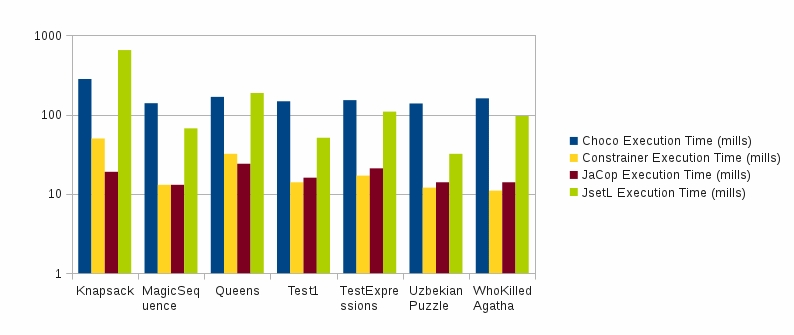
\includegraphics[scale=.45]{img/grafico11.jpg}
\caption{test semplici, tempo impiegato.}
\end{figure}

Come si evince in figura, in questi semplici test JSetL si comporta abbastanza
bene, meglio di Choco in ben cinque casi su sette e praticamente un pareggio
sul problema delle otto regine. Si potrebbe dire che con poche variabili
l'ordine di grandezza del tempo impiegato coincide con Choco. Il discorso è
differente se si confronta con Constrainer o JaCoP, decisamente più performanti.

\begin{figure}[!ht]
\centering
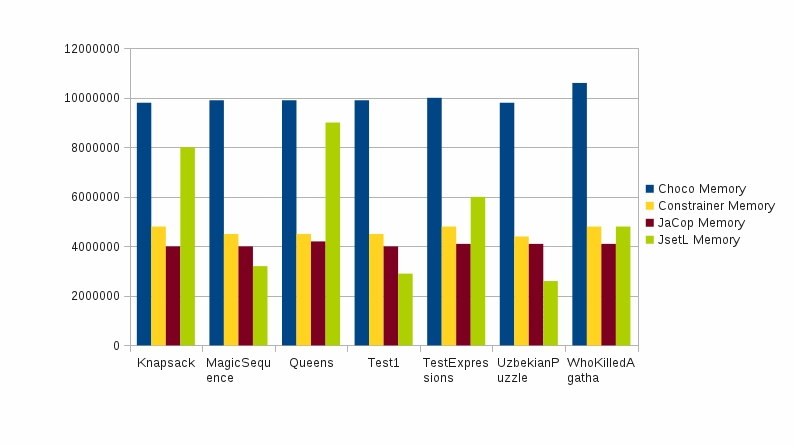
\includegraphics[scale=.45]{img/grafico12.jpg}
\caption{test semplici, memoria utilizzata.}
\end{figure}
Per quanto riguarda la memoria utilizzata invece, JSetL riesce ad essere
sempre sotto ai livelli di Choco e ben tre volte meglio di tutti gli altri.
I casi in cui viene utilizzata tanta memoria sono \emph{Knapsack} e
\emph{Queen}. Il primo probabilmente è causato dalla ricerca ottima
(\texttt{findOptimalSolution}), che non è direttamente supportata dal solver
JSetL, ma viene implementata mediante un algoritmo fatto ad \emph{hoc} che
espande e
propaga un vincolo all'interno del solver. Mentre la pesantezza
del problema delle regine, in termini di
memoria,  è indubbiamente dovuto alla presenza del
vincolo AllDifferent su tante variabili, e come questo è implementato in JSetL.

\subsection{Test complessi}
I test più complessi sono caratterizzati da un elevato numero di variabili
legate al problema o di supporto e da un elevato numero di vincoli, su tutti
quelli globali: Cardinality, AllDifferent, etc.

Sono stati catalogati come complessi poiché anche i solver che hanno dato prova
di essere i più performanti (JaCoP e Constrainer) risolvono i problemi dati
con tempi ben al di sopra dei precedenti.


Dal grafico si può notare che JSetL in questi casi è ben al di sopra degli altri
solver come tempo d'esecuzione. Nel test \emph{Golomb Rulers} il tempo
impiegato è circa il doppio rispetto a Choco e il triplo rispetto JaCoP e
Constrainer. In \emph{Magic Square} è ben dieci volte più lento degli altri,
mentre in \emph{Graph Coloring} circa sessanta. In questo caso però occorre dire
che JaCoP sembra non terminare, infatti la sua barra non è presente nel grafico.

\begin{figure}[!ht]
\centering
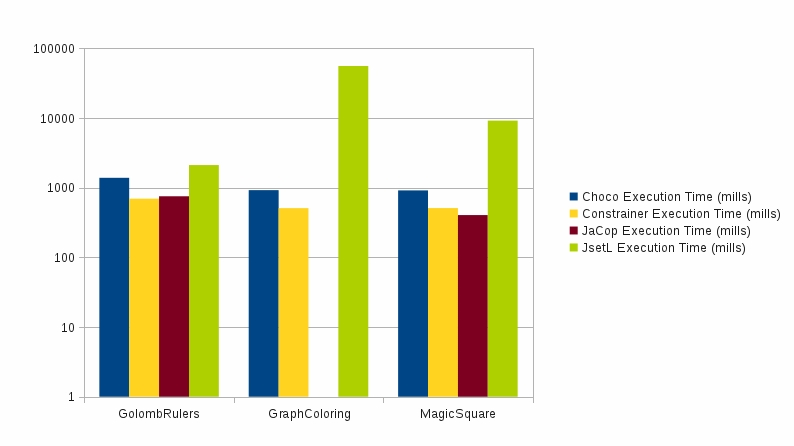
\includegraphics[scale=.45]{img/grafico13.jpg}
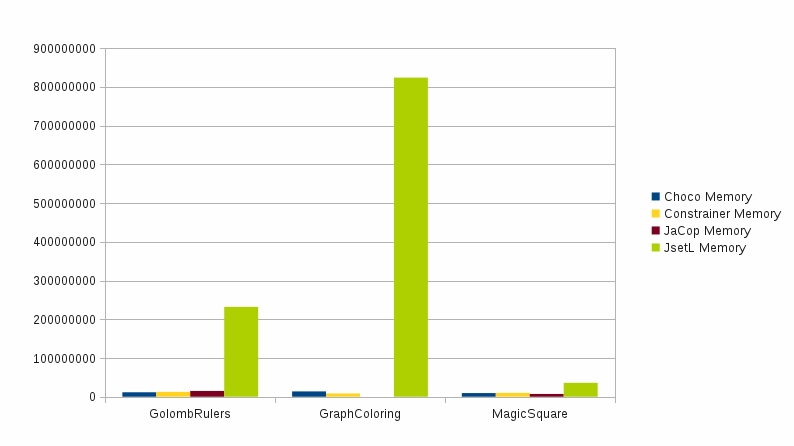
\includegraphics[scale=.4]{img/grafico14.jpg}
\caption{test complessi.}
\end{figure}

Per quanto riguarda la memoria utilizzata nei test complessi è invece evidente
che JSetL ne utilizzi veramente troppa rispetto agli altri solver e molto
probabilmente anche il deficit di prestazioni è dovuto a questo.

